% !TEX root = mythesis.tex

%==============================================================================
\chapter{Data Analysis and Discussion}
\label{sec:data_analysis}
%==============================================================================
\section{Image Inspection and galaxy distribution}\label{sec:image_inspection}
%
A contour plot of the corrected and cheese-masked wavelet-filtered image is shown in Figure \ref{fig:contour_wvl_filtered} to visualize emission beyond \(R_{500}\) more clearly. Furthermore, the galaxy distribution using data from NASA/IPAC Extragalactic Database (NED) is extracted within a \(\SI{1}{\degree}\) radius of the galaxy group NGC 1550 and overlayed. There are 26 galaxies with similar redshifts \(0.010 \leq z \leq 0.015\) including the galaxy NGC1550 (\(z=0.0123\)) itself. From Figure \ref{fig:contour_wvl_filtered} it is clear that the group appears spherically symmetrical and relaxed, with a distinct emission cutoff visible at \(R_{500}\). Beyond this radius, emission becomes difficult to distinguish from the background, which is fairly complex due to the Orion-Eridanus superbubble (cf. Section \ref{sec:background}). There is a noticeable gradient in the background emission, with a lower background to the north compared to the south. The galaxy distribution is loosely clustered to the northeast, but no clear correlation with the X-ray contours is observed. Usually, this helps indicate whether excess emission along a certain direction is significant.

To highlight emission structures within \(R_{500}\), Figure \ref{fig:contour_fully_corrected} presents a contour plot of the corrected soft-band image smoothed with a Gaussian kernel of \(8\) pixels. Within this radius, some deviations from perfect azimuthal symmetry are noticeable. A slight east-west elongation within approximately \(390''\) (inner circle in the figure) can indeed be inferred as mentioned in Section \ref{sec:ngc1550}. Beyond \(390''\), features are harder to distinguish: the emission in the north, south and east appear slightly more irregular. Emission in the west, falls more uniformly and there seems to be slight emission dip between \(390''\) and \(810''\) (outer circle in the figure) compared to the other sectors.
\begin{figure}[htbp]
    \centering
    \includegraphics{data_analysis/galaxy_distribution.pdf}
    \caption{Contour plot of the corrected, cheese-masked, wavelet-filtered image with overlaid galaxy distribution (red crosses) within a \(\SI{1}{\degree}\) radius of NGC 1550. The color bar represents counts per second. The plot shows a distinct emission boundary at \(R_{500}\), with emission beyond this radius becoming difficult to distinguish from the background. The galaxy distribution is clustered to the northeast, though no clear correlation with the X-ray contours is observed.}
    \label{fig:contour_wvl_filtered}
\end{figure}
\begin{figure}[htbp]
    \centering
    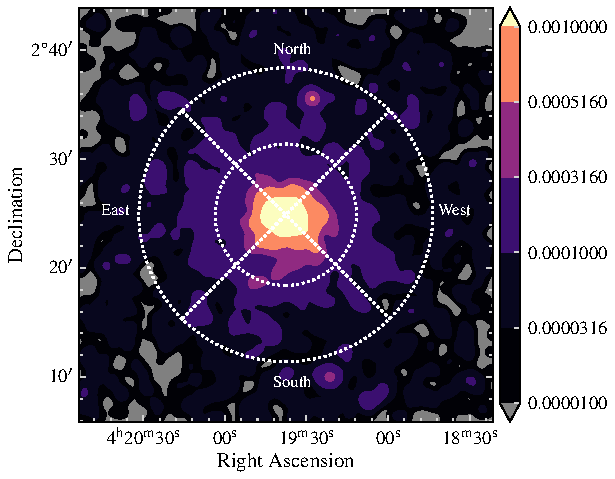
\includegraphics{data_analysis/countour_plot_corr_R500.pdf}
    \caption{Contour plot of the corrected soft-band image smoothed with a Gaussian kernel of 8 pixels. The color bar indicates counts per second. Some deviations from azimuthal symmetry are observed within the outer circle (\(\sim 810''\)). The inner circle denotes a radius of \(\sim 390''\). Within this region, an east-west elongation of the core is noticeable. The four wedges labeled north, south, east, and west correspond to the angular (but not radial) ranges used to extract surface brightness.}
    \label{fig:contour_fully_corrected}
\end{figure}
\section{Full Azimuthal Surface Brightness Profile}\label{sec:full_az}
To more accurately identify or exclude potential deviations from spherical symmetry, surface brightness (SB) analysis will be performed. First, the emission center is estimated by constructing a \(2'\) aperture around the apparent center (right ascension \SI{64.9066}{\degree} and a declination \SI{2.4151}{\degree}). This aperture size is chosen to capture a statistically significant number of photons without leaving the group center. The flux-weighted average coordinates of the fully corrected image within this aperture yields a right ascension of \SI{64.909}{\degree} and a declination of \SI{2.414}{\degree} and shall be referred to as the SB-center. Concentric anulli of \(1'\) width are constructed from the SB-center up to to an angular distance of \(80' \approx 1.5R_{200}\). The counts \(C\) within each annulus are determined using the \texttt{funcnts} task from the \texttt{funtools} software, with a Poisson error of \(\sqrt{C}\). The surface brightness \(S\) for each annulus is calculated by
\begin{align*}
    S = \frac{C_\text{filt} - C_\text{PIB}}{C_\text{expmap}\cdot A},
\end{align*}
where \(C\) denotes the counts in the filtered photon image, total PIB map, and exposure map, respectively, and \(A\) is the annulus area. Errors are calculated using Gaussian error propagation. Furthermore, background estimation is performed using \(10\) circular regions with a \(30'\) radius, each centered at a distance of \(100'\) from the SB-center (Figure \ref{fig:background_circles}). The average background surface brightness is evaluated for all circles combined and separately for the northern (Circles 1-5) and southern region (Circles 6-10) to account for the background gradient. Table \ref{tab:background} lists the average background for all 3 cases. As is clear from the table, the total background level is consistent with the other two within \(1\sigma\). Therefore, unless otherwise specified, the total background value derived from all circles will be used for the subsequent analysis and interpretation.
%
\begin{figure}[htbp]
    \centering
    \includegraphics{data_analysis/_background.pdf}
    \caption{Background estimation. Depicted are 10 circular regions utilized to estimate the observed background. Circles 1-5 correspond to the northern background, and Circles 1-6 to the southern background. The total background corresponds to all circular regions. The obtained values can be found in Table \ref{tab:background}.}
    \label{fig:background_circles}
\end{figure}
%
\begin{table}[htbp]
    \centering
    \begin{tabular}{l c}
    \toprule
    Region & Background / cts s$^{-1}$ arcsec$^{-2}$ \\
    \midrule
    North & $(1.03 \pm 0.10) \times 10^{-7}$ \\
    South & $(1.27 \pm 0.04) \times 10^{-7}$ \\
    Total & $(1.15 \pm 0.14) \times 10^{-7}$ \\
    \bottomrule
    \end{tabular}
    \caption{Surface brightness and associated errors for the different background regions.}
    \label{tab:background}
\end{table}
%

A \(\beta\)-model (cf. Section \ref{sec:beta_model}) is employed to characterize the surface brightness profile, given by
\begin{align*}
    S_X(r) = S_X(0)\left(1 + \left(\frac{r}{r_c}\right)^2\right)^{-3\beta + 0.5} + d
\end{align*}
where \(d\) represents the background emission. The center of each annulus is taken to be \(r\) and the corresponding surface brightness values are utilized. The optimized parameters and \(\chi^2 / \text{d.o.f}\) (chi squared per degrees of freedom) are listed in Table \ref{tab:full_az_fit_parameters}. Figure \ref{fig:tot_azimuthal_beta_model} illustrates the surface brightness as a function of radial distance from the center, including both the fitted \(\beta\)-model and the observationally estimated background level.
\begin{figure}[htbp]
    \centering
    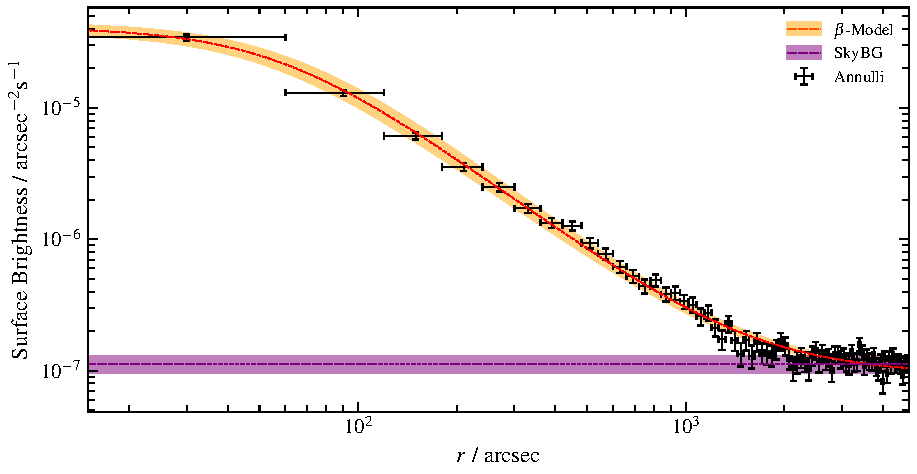
\includegraphics{data_analysis/beta_motel_tot_surf_bri_anulli1_1arcmin.pdf}
    \caption{Surface Brightness within each annulus (black crosses) as a function of distance from the determined SB-center including error bars. The dashed orange line represents the best \(\beta\)-model fit, while the purple line indicates the observationally determined background. The shaded regions correspond to their respective \(1\sigma\) intervals.}
    \label{fig:tot_azimuthal_beta_model}
\end{figure}
\begin{table}[htbp]
    \centering
    \begin{tabular}{lcccc}
    \toprule
    Parameter & $S_0$ / cts s$^{-1}$ arcsec$^{-2}$ & $\beta$ & $r_c$ / \(''\) & $d$ / cts s$^{-1}$ arcsec$^{-2}$ \\
    \midrule
        & $(4.1 \pm 0.4) \times 10^{-5}$ & $0.478 \pm 0.008$ & $60 \pm 5$ & $(9.3 \pm 0.4) \times 10^{-8}$ \\
    \midrule
    \(\chi^2 / \text{d. o. f}\) & \multicolumn{4}{c}{0.96} \\
    \bottomrule
    \end{tabular}
    \caption{Fit parameters, their errors, and the reduced chi-squared value for the full azimuthal surface brightness profile.}
    \label{tab:full_az_fit_parameters}
\end{table}

The \(\beta\)-model fit for the surface brightness profile, shown in Figure \ref{fig:tot_azimuthal_beta_model}, yields \(\beta = \num{0.478\pm0.008}\) and a core radius \(r_c = (\num{60\pm5})'' \approx (15\pm2)\,\text{kpc}\) with \(\chi^2/\text{d.o.f.} = 0.96\). This result is consistent with previous studies: \citep{Kawaharada_2003} report \(\beta = 0.47\) and \(r_c \approx (16\pm1)\,\text{kpc}\) using ASCA data; \citep{Kawaharada_2009} use a double \(\beta\)-model to find \(\beta = \num{0.50\pm0.05}\) and \(r_c \approx (20\pm3)\,\text{kpc}\) for the outer component from XMM-Newton data; \citep{Sun_2003} also derive \(\beta \sim 0.48\) and a slightly higher \(r_c \approx 26\,\text{kpc}\) for the outer component using Chandra data; \citep{Reiprich_2002}, although, report a somewhat higher \(\beta = 0.554^{+0.049}_{-0.037}\) using ROSAT. The surface brightness profile also highlights that the group emission decreases to the background level at approximately \(R_{500}\), as observed in Section \ref{sec:image_inspection}. The observationally estimated total background in Table \ref{tab:background}, however, is approximately 24\% higher than the background obtained by the \(\beta\)-model fit (cf. Table \ref{tab:full_az_fit_parameters}) at \(1.5\sigma\). Although this discrepancy is not too alarming, it does indicate challenges associated with the complex background, implying that they could have been chosen more carefully.

A double \(\beta\)-model fit was not successful. This can be attributed to the angular resolution of the \(1'\) width anulli, limiting the ability to resolve the inner core emission. Performing a \(\beta\)-model fit with finer annuli was attempted, but this did not significantly improve the description of the surface brightness profile within the core and resulted in poor error estimation in the outskirts due to low count rates. Indeed, \citep{Kawaharada_2009} find an inner core component of \(r \sim 3\,\text{kpc}\) corresponding to \(\approx 12'' \) which is comparable to the eROSITA angular resolution \(\sim 15''\) (\cite{Predehl2021}). A successful two-\(\beta\) model, however, might be possible by fixing the inner core radii or convolving the model with the eROSITA point spread function, but this was not attempted within the scope of this thesis.
\subsection{\(\beta\)-Model and Residual Image}
Using the parameters from Table \ref{tab:full_az_fit_parameters}, a \(\beta\)-model image (Fig. \ref{fig:beta_model}) and a residual image (Fig. \ref{fig:residual_image}) are created. The \(\beta\)-model image is generated by distributing the one-dimensional \(\beta\)-model across the image. This involves computing the distance from the surface brightness center to each coordinate \((x, y)\) in the image and then scaling the output of the \(\beta\)-model by the eROSITA pixel area of \(16\text{arcsec}^2\). The residual image (res. img) was obtained by subtracting the scaled \(\beta\)-model from the corrected soft-band image (corr. img). Hence,
\begin{align*}
    \text{res. img}(x, y) = \text{corr. img}(x, y) - S\left(\sqrt{x^2 + y^2}\right) \cdot \text{pix. area}.
\end{align*}

The residual image indicates that the \(\beta\)-model overestimates emission within \(R_{500}\), while underestimating emission at the center significantly (highlighted by a green arrow in Figure \ref{fig:residual_image}). The latter can be attributed to the absence of a second \(\beta\)-component, as a single \(\beta\)-model often inadequately describes the inner core emission, which is often higher-than-expected. \citep{Sun_2003} report, however, that even a two \(\beta\)-fit is not sufficient to describe the surface brightness within the central \(1\,\text{kpc}\). Disregarding the excess emission within the core, no significant substructure or features can be noticed from the residual image.
\begin{figure}[htbp]
    \centering
    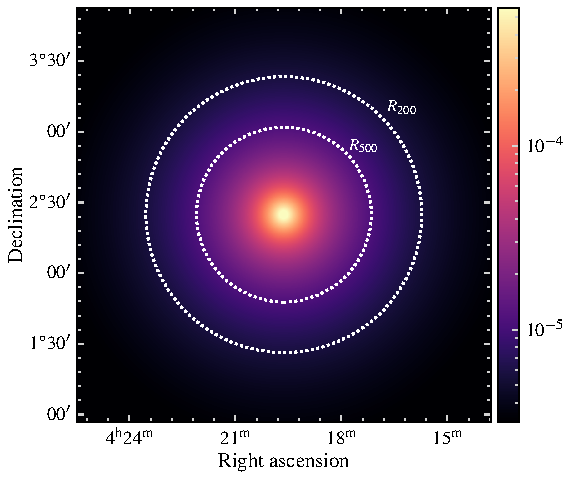
\includegraphics{data_analysis/beta_model.pdf}
    \caption{\(\beta\)-model image of NGC1550 utilizing the parameters in \ref{tab:full_az_fit_parameters}. The color bar represents counts per second.}
    \label{fig:beta_model}
\end{figure}
\begin{figure}[htbp]
    \centering
    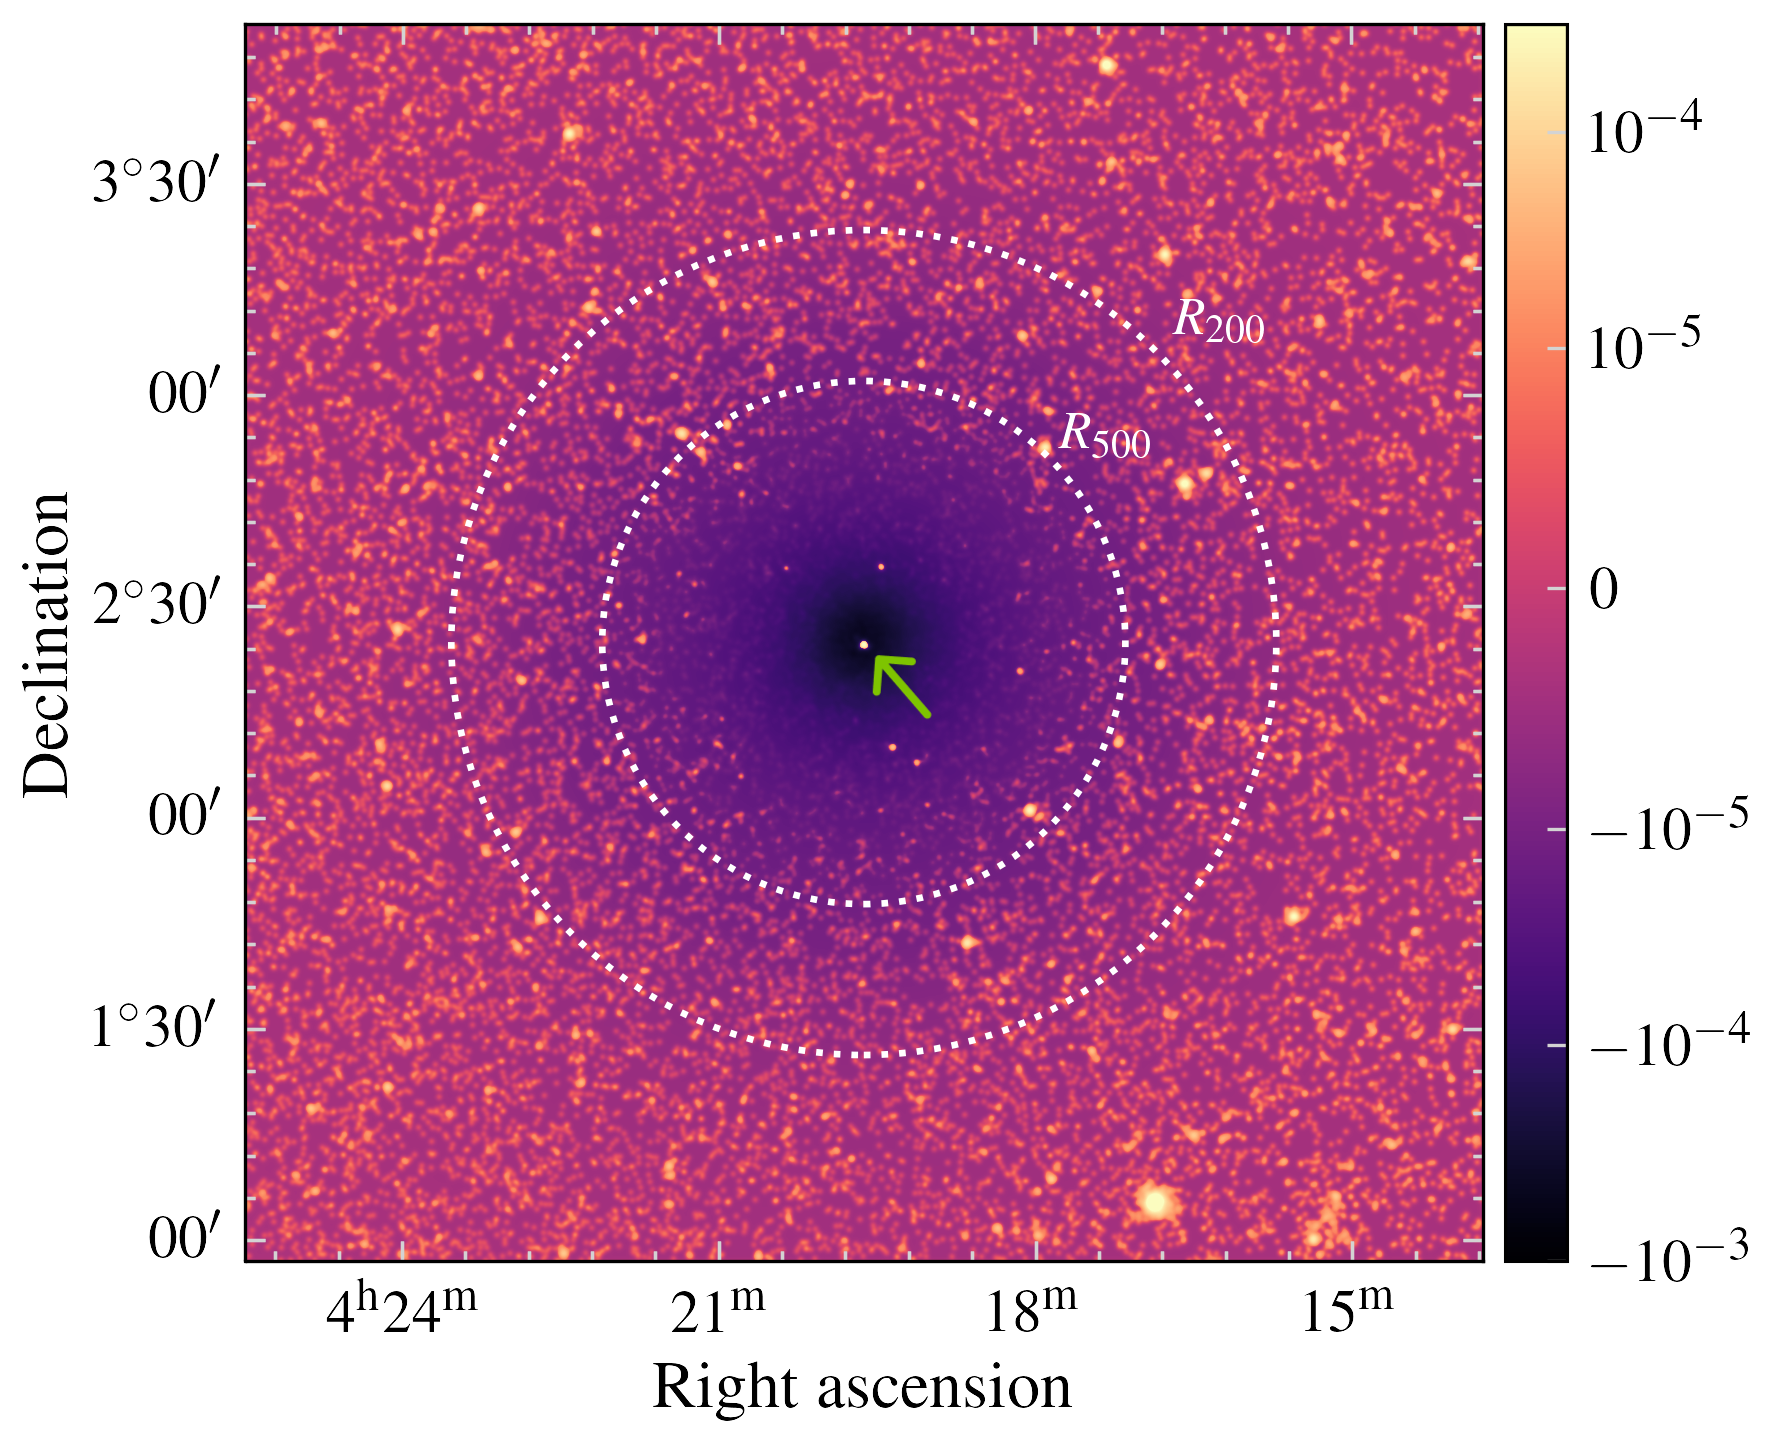
\includegraphics{data_analysis/residual_image.png}
    \caption{Residual image of NGC1550 derived by subtracting \(\beta\)-model image from the corrected soft-band image. The color bar represents counts per second and the image has been smoothed with a Gaussian-kernel of 5 pixels. The residual image indicate that the \(\beta\)-model slightly overestimates the emission around the core, due to the inadequacy of a single \(\beta\)-model in capturing the core's emission.}
    \label{fig:residual_image}
\end{figure}
\section{Sectoral Surface Brightness Analysis}
Thus far, the surface brightness analysis has encompassed the entire azimuthal extent of the group. By analyzing surface brightness within specific sectors and comparing them to the full azimuthal profile, elongation in certain directions can be revealed. Various authors have reported an east-west elongation at the center of NGC1550 (\cite{Sun_2003}, \cite{Kolokythas_2020}), making it particularly interesting to determine whether this elongation extends into the outer regions of the group. To investigate this, four sectoral regions (north, south, east, and west) are divided into annuli, as shown in Figure \ref{fig:contour_fully_corrected}. The center, width and extension of the annuli remain as described in Section \ref{sec:image_inspection}, and surface brightness calculations and \(\beta\)-model fitting follow the same methodology.

Each region is initially fitted individually. Thereafter, the north and south sectors are combined for fitting, as are the east and west sectors. Figure \ref{fig:beta_model_West_East} illustrates the comparison between the east and west profiles and Figure \ref{fig:beta_model_North_South} compares the north and south profiles. The top graph in each figure shows the surface brightness profiles, including the observationally determined sky background and the corresponding \(\beta\)-model. The lower two graphs display the relative surface brightness differences of each region (\(\text{SB}_\text{sec}\)) compared to the full azimuthal surface brightness profile (\(\text{SB}_\text{an}\)). The error bars represent the error of the relative difference computed by Gaussian error propagation. The fit parameters for each \(\beta\)-model are listed in Table \ref{table:full_sec_fit_parameters}. 

The fits are of lower quality when compared to the full azimuthal \(\beta\)-model fit ($\chi^2 / \text{d.o.f.} \lesssim 0.8$), suggesting possible overfitting or, more likely, an overestimation of the errors as attempts using wider $2'$ annuli resulted in significantly improved $\chi^2 / \text{d.o.f.} \gtrsim 0.95$ for the west, north, and combined east-west profiles, and a modest improvement for the remaining sectors. However, since the full azimuthal analysis was only performed with the smaller annuli and the resulting fit parameters were similar across both cases, the smaller annuli will be utilized for the following comparison. 

When inspecting the western region, the emission dip observed in the western region between approximately \(390''\) and \(810''\) -- as noted in section \ref{sec:image_inspection} -- is noticeable in relation to the full azimuthal surface brightness profile. However, these deviations are not quantitatively significant and may be attributed to statistical fluctuations. For the northern and southern sectors, a significant deviation is noted at the first data point. This discrepancy is likely due to a suboptimal choice of the SB-center and is probably not physically significant, which shall be elaborated further below. In all sectors, however, no notable deviation from the full azimuthal profile is observed beyond \(390'\). The combined east-west and north-south emissions are compared in Figure \ref{fig:beta_model_East_West_North_South} with the \(\beta\)-model parameters being listed in Table \ref{table:full_sec_fit_parameters}. Here, too, no significant deviation from the full azimuthal profile is observed beyond the first data points, indicating that the east-west elongation observed within \(390''\) in Section \ref{sec:image_inspection} does not extend towards the outskirts of the group. The east-west elongation whithin \(390''\) can not be quantitatively confirmed, as only the third annulus shows an appreciable deviation compared to the combined north-south profile. This is complicated further by the potentially missplaced SB-center (\textit{vide infra}) and the wide annuli, which set an arbitrary data resolution. 
\begin{figure}[htbp]
    \centering
    \begin{subfigure}{\textwidth}
        \centering
        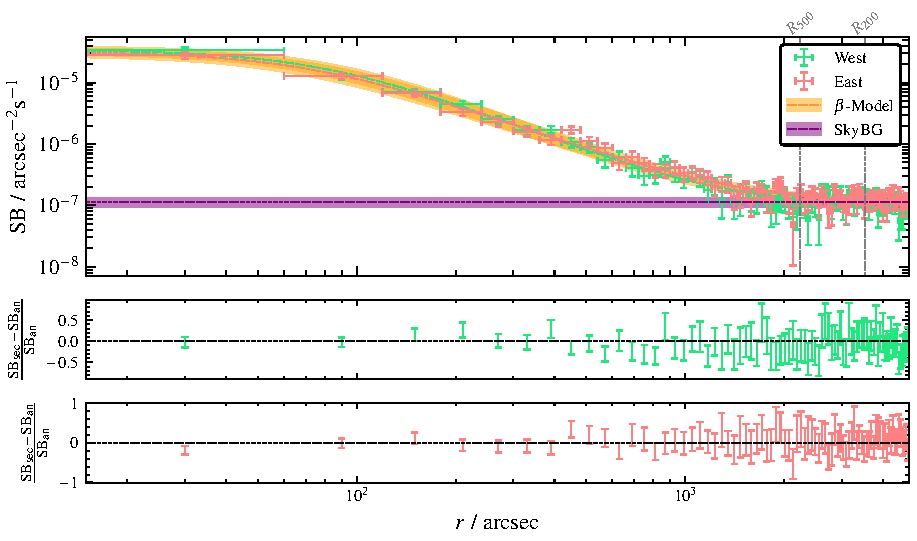
\includegraphics{data_analysis/beta_model_West-East.pdf}
        \caption{\(\beta\)-model fits for the West and East regions.}
        \label{fig:beta_model_West_East}
    \end{subfigure}
    \vspace{0.5cm} 
    \begin{subfigure}{\textwidth}
        \centering
        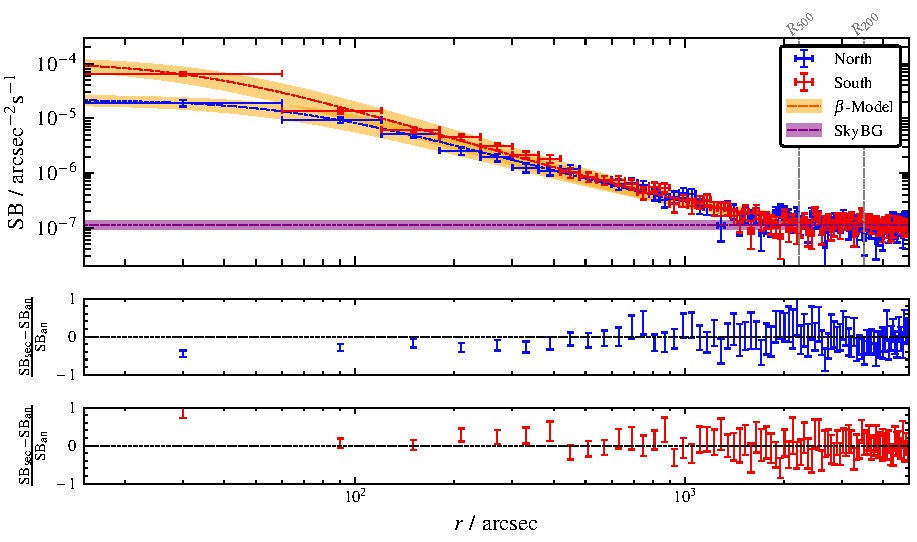
\includegraphics{data_analysis/beta_model_North-South.pdf}
        \caption{\(\beta\)-model fits for the North and South regions.}
        \label{fig:beta_model_North_South}
    \end{subfigure}
    \caption{\(\beta\)-model fits for the West-East and North-South regions. \textit{Top of each panel:} Surface brightness profiles, including the observationally determined sky background. \textit{Bottom of each panel:} Relative surface brightness differences between each region (\(\text{SB}_{\text{sec}}\)) and the full azimuthal surface brightness profile (\(\text{SB}_{\text{an}}\)).}
    \label{fig:beta_models_West_North}
\end{figure}
%
\begin{figure}[htbp]
    \centering
    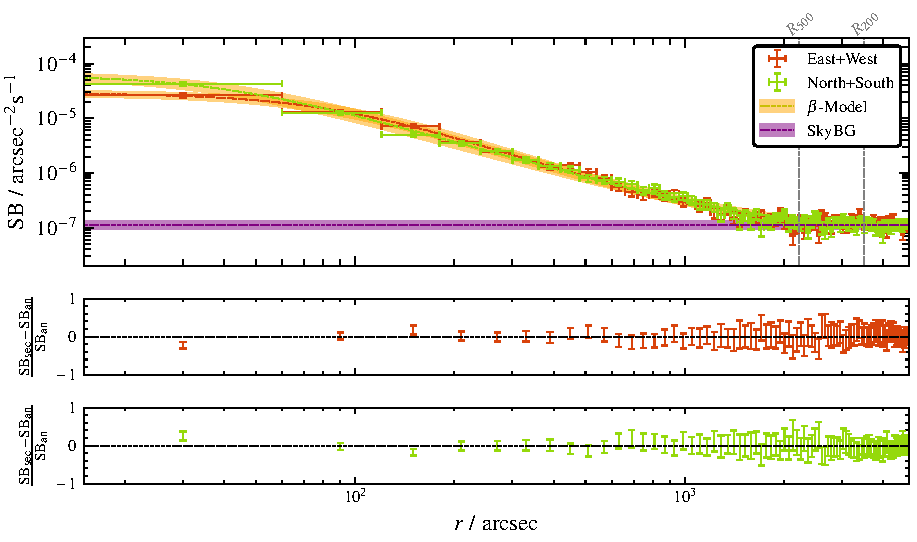
\includegraphics{data_analysis/beta_model_East+West-North+South.pdf}
    \caption{\(\beta\)-model fits for the combined east-west and north-south regions. The surface brightness profile is show in the top graph and the lower two graphs display the relative surface brightness differences between each region (\(\text{SB}_{\text{sec}}\)) and the full azimuthal surface brightness profile (\(\text{SB}_{\text{an}}\)). Error bars are derived from Gaussian error propagation. Excluding the first data point, both combined surface brightness profiles show no significant deviation from the full azimuthal profile and are entirely consistent with each other, indicating no significant east-west elongation in the outskirts of the galaxy group.}
    \label{fig:beta_model_East_West_North_South}
\end{figure}
%
\begin{table}[htbp]
    \centering
    \resizebox{\textwidth}{!}{%
        \begin{tabular}{lccccc}
        \toprule
        Parameter & $S_0$ / cts s$^{-1}$ arcsec$^{-2}$ & $\beta$ & $r_c$ / $''$ & $d$ / cts s$^{-1}$ arcsec$^{-2}$ & $\chi^2 / \text{d. o. f}$ \\
        \midrule
        East-West & \((2.88 \pm 0.27) \times 10^{-5}\) & \((5.08 \pm 0.12) \times 10^{-1}\) & \((8.60 \pm 0.80) \times 10^{1}\) & \((1.02 \pm 0.05) \times 10^{-7}\) & \(0.83\)\\
        North-South & \((6.20 \pm 0.71) \times 10^{-5}\) & \((4.58 \pm 0.07) \times 10^{-1}\) & \((4.01 \pm 0.43) \times 10^{1}\) & \((8.45 \pm 0.46) \times 10^{-8}\) & \(0.71\)\\
        West & \((3.42 \pm 0.42) \times 10^{-5}\) & \((5.20 \pm 0.16) \times 10^{-1}\) & \((8.11 \pm 0.98) \times 10^{1}\) & \((9.63 \pm 0.60) \times 10^{-8}\) & \(0.77\)\\
        East & \((3.18 \pm 0.43) \times 10^{-5}\) & \((4.87 \pm 0.15) \times 10^{-1}\) & \((7.22 \pm 0.97) \times 10^{1}\) & \((1.02 \pm 0.07) \times 10^{-7}\) & \(0.82\)\\
        North & \((2.23 \pm 0.35) \times 10^{-5}\) & \((4.49 \pm 0.14) \times 10^{-1}\) & \((6.6 \pm 1.1) \times 10^{1}\) & \((7.89 \pm 0.78) \times 10^{-8}\) & \(0.78\)\\
        South & \((1.10 \pm 0.20) \times 10^{-4}\) & \((4.69 \pm 0.10) \times 10^{-1}\) & \((3.32 \pm 0.53) \times 10^{1}\) & \((8.69 \pm 0.64) \times 10^{-8}\) & \(0.86\)\\
        \bottomrule
        \end{tabular}
    }
    \caption{Fit parameters, their errors, and the reduced chi-squared value for the \(\beta\)-model fit of the north, south, east and west sectors and the combined north-south and east-west sectors.}
    \label{table:full_sec_fit_parameters}
\end{table}
%

It is notable that the \(\beta\) parameter and the core radius \(r_c\) are not always consistent when comparing the sectors against each other and with the full azimuthal profile. For example, the core radius \(r_c\) for the combined east-west region is more than twice as large as that for the combined north-south region, and the \(\beta\) value is approximately \(10\%\) larger, with discrepancies at \(> 5\sigma\) and \(> 3\sigma\), respectively. In fact, most of the \(\beta\)-values and core radii are inconsistent within \(1\sigma\) when comparing the sectors against each other. This discrepancy may indicate a poor SB-center choice, which is biasing the surface brightness towards the south. For instance, the southern sector's normalization factor \(S_0\) shows a relative difference of almost \(80\%\) compared to the north sector, with a \(4.32\sigma\) deviation. Consequently, the estimated SB-center at \(\SI{64.909}{\degree}\) and \(\SI{2.414}{\degree}\) is likely too far north, leading to an overestimation of southern emission in the initial data points, which is clearly visible in Figure \ref{fig:beta_model_North_South}. This issue is probably exacerbated by the wide \(1'\) annuli, meaning that excess emission of the first data point might be significantly affecting the fits. 

Regarding the background, the fitted background level is in agreement with the total background level for the east, west and combined east-west regions. However, for the north and south regions, the fitted background level underestimates the observationally determined north and south backgrounds by \(31\%\) and \(46\%\), at \(1.9\sigma\) and \(0.98\sigma\), respectively. This discrepancy might be simply due to the inherently complex background of the Orion-Eridanus superbubble, though it can also be taken as an indication that the circles chosen for background estimation in Figure \ref{fig:background_circles} are not far enough from the SB-center.

In general, such deviations in fit parameters would align well with the common notion that galaxy groups never exhibit perfect azimuthal symmetry, since infalling matter inevitably causes irregularities. Due to the aforementioned issue regarding the SB-center, one can not conclusively take the fit deviations of the sectoral surface brightness analysis as confirmation for this view. Regardless, the sectoral surface profiles confirm that no significant deviations from azimuthal symmetry can be established in the outskirts, were the above mentioned issues of the SB-center and annuli width are largely insignificant, and contamination from the background dominates.

